\section{Архитектуры вычислительных сетей}

Вычислительные системы имеют два основных вида построения архитектуры: централизованный
и распределенный (также называемый клиент-сервер).

Основное различие между ними состоит в том, что в централизованной архитектуре большая
часть вычислений происходит на сервере. В распределенной системе все машины имеют
одинаковое назначение и все занимаются вычислениями.

Система клиент-сервер состоит из двух типов взаимодействующих устройств (см.
рисунок~\ref{pic:client-server}).
В большинстве случаев взаимодействие происходит по следующей модели:

\begin{enumerate}
    \item Клиент отправляет запрос на получение данных серверу;
    \item Сервер, получив запрос, начинает обработку данных, различные расчеты и т.п.
        (в зависимости от назначения сервера);
    \item Сервер отправляет обработанные или новые данные клиенту.
\end{enumerate}

\begin{figure}[h]
    \center
    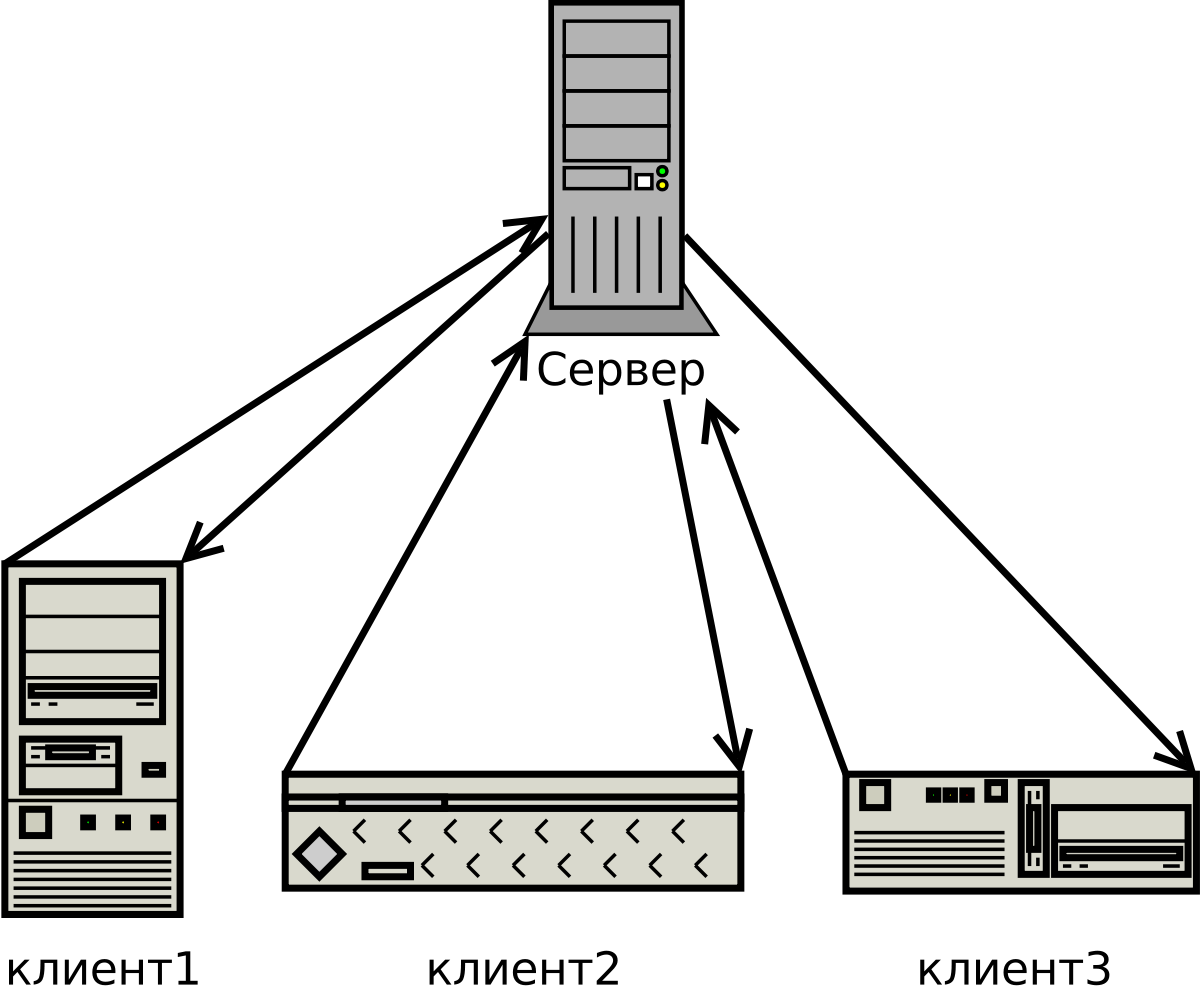
\includegraphics[height=9cm]{client-server}
    \caption{Клиент-серверная архитектура}
    \label{pic:client-server}
\end{figure}

\begin{figure}[h]
    \center
    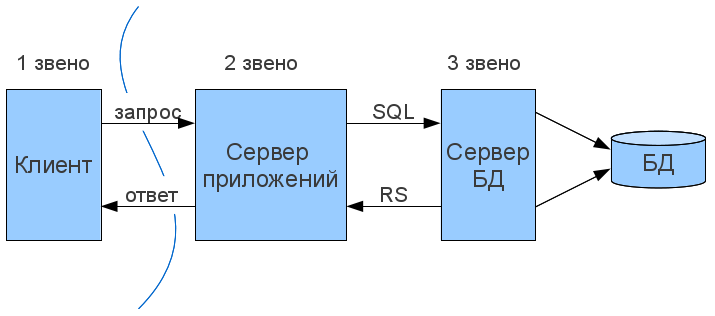
\includegraphics[height=5cm]{client-server-db}
    \caption{Клиент-серверная архитектура с разделением серверов}
    \label{pic:client-server-db}
\end{figure}

В настоящее время в сетях с централизованной архитектурой может быть применен принцип
разделения обязанностей серверов. Например, разделение серверов приложений, баз данных и
вычислений (см. рисунок~\ref{pic:client-server-db}).

